\documentclass{beamer}
\usepackage{tikz,amsmath,hyperref,graphicx,stackrel,animate,amssymb}
\usetikzlibrary{positioning,shadows,arrows,shapes,calc}
\newcommand{\argmax}{\operatornamewithlimits{argmax}}
\newcommand{\argmin}{\operatornamewithlimits{argmin}}
\mode<presentation>{\usetheme{Frankfurt}}
\AtBeginSection[]
{
  \begin{frame}<beamer>
    \frametitle{Outline}
    \tableofcontents[currentsection,currentsubsection]
  \end{frame}
}
\title{Lecture 24: Pitch Tracking}
\author{Mark Hasegawa-Johnson}
\date{ECE 401: Signal and Image Analysis}
\begin{document}

% Title
\begin{frame}
  \maketitle
\end{frame}

% Title
\begin{frame}
  \tableofcontents
\end{frame}

%%%%%%%%%%%%%%%%%%%%%%%%%%%%%%%%%%%%%%%%%%%%%%%%%%%%%%%%%%%%%%%%%%%%%%%%%%%%%%
\section[Review]{Review: Autocorrelation and Covariance}

\begin{frame}
  \frametitle{Review: Autocorrelation and Covariance}

  \begin{itemize}
  \item Autocorrelation:
    \begin{align*}
      r_x[n] = \sum_{m=-\infty}^\infty x[m]x^*[m-n]
    \end{align*}
  \item If the signal is stationary and zero-mean, then autocorrelation
    is a scaled estimate of covariance:
    \begin{align*}
      \rho_x[m,m-n] &=E\left[(x[m]-\mu_x[m])(x[m-n]-\mu_x[m-n])^*\right]
    \end{align*}
  \item Autocorrelation is flipped convolution:
    \begin{align*}
      r_x[n] = x[n]\ast x^*[-n]
    \end{align*}
  \item Power spectrum is the DTFT of convolution:
    \begin{align*}
      \mathcal{F}\left\{r_x[n]\right\}
      &=|X(\omega)|^2
    \end{align*}
  \end{itemize}
\end{frame}
    
\begin{frame}
  \frametitle{Example: White Noise}

  \begin{itemize}
  \item For example, \textbf{white noise} is a signal whose samples
    are completely uncorrelated with each other:
    \begin{align*}
      E\left[r_x[n]\right] &= E\left[x[m]x^*[m-n]\right]\\
      &= \delta[n]
    \end{align*}
  \item This is called white noise because its Fourier transform has
    equal energy at all frequencies, like white light:
    \begin{align*}
      E\left[|X(\omega)|^2\right] &=
      \mathcal{F}\left\{\delta[n]\right\}\\ &= 1
    \end{align*}
  \end{itemize}
\end{frame}

%%%%%%%%%%%%%%%%%%%%%%%%%%%%%%%%%%%%%%%%%%%%%%%%%%%%%%%%%%%%%%%%%%%%%%%%%%%
\section[Exponential]{Autocorrelation and power spectrum of a windowed complex exponential}

\begin{frame}
  \frametitle{Autocorrelation of a windowed complex exponential}

  Suppose that $x[n]=w[n]e^{j\omega_0 n}$.  
  What is its autocorrelation?
  \begin{align*}
    r_x[n] &= \sum_{m=-\infty}^\infty w[m]e^{j\omega_0 m}w^*[m-n]e^{-j\omega_0(m-n)}\\
    r_x[n] &= e^{j\omega_0 n}\sum_{m=-\infty}^\infty w[m]w^*[m-n]\\
    &= e^{j\omega_0 n} r_w[n]
  \end{align*}
  \begin{itemize}
    \item The autocorrelation of a windowed complex exponential is a
      windowed complex exponential!
    \item The autocorrelation is windowed by $r_w[n]$, the
      autocorrelation of $w[n]$
  \end{itemize}
\end{frame}

\begin{frame}
  \frametitle{Power spectrum of a windowed complex exponential}

  \begin{align*}
    x[n]=w[n]e^{j\omega_0 n} &\Rightarrow r_x[n]=e^{j\omega_0 n} r_w[n]
  \end{align*}
  What is its power spectrum?
  \begin{align*}
    X(\omega) &= W(\omega-\omega_0)\\
    |X(\omega)|^2 &= |W(\omega-\omega_0)|^2
  \end{align*}
\end{frame}
    
%%%%%%%%%%%%%%%%%%%%%%%%%%%%%%%%%%%%%%%%%%%%%%%%%%%%%%%%%%%%%%%%%%%%%%%%%%%
\section[Cosine]{Autocorrelation and power spectrum of a windowed cosine}

\begin{frame}
  \frametitle{Autocorrelation of a windowed cosine}

  \begin{itemize}
  \item Suppose that $x[n]=w[n]\cos(\omega_0 n)$.  What is its autocorrelation?
    \begin{align*}
      r_x[n] &= \sum_{m=-\infty}^\infty w[m]\cos(\omega_0 m)w^*[m-n]\cos(\omega_0(m-n))
    \end{align*}
  \item WARNING: AUTOCORRELATION IS NOT LINEAR!  For DTFT we used the
    relationship $\cos(\omega
    n)=\frac{1}{2}(e^{j\omega{n}}+e^{-j\omega{n}})$ to make the
    problem easy, but that won't work for autocorrelation, because
    it's not linear.
  \item \ldots but we can use a trig identity to help us:
    \begin{align*}
      &\cos(a)\cos(b)  =\frac{1}{2}\left(\cos(a+b)+\cos(a-b)\right)\\
      &\sum_m w[m]w^*[m-n]\cos(\omega_0m)\cos(\omega_0(m-n)) =\\
      &\sum_m w[m]w^*[m-n]\frac{1}{2}\left(\cos(\omega_0(2m-n))+\cos(\omega_0 n)\right)
    \end{align*}
  \end{itemize}
\end{frame}

\begin{frame}
  \frametitle{Autocorrelation of a windowed cosine}

  \begin{align*}
    &x[n] =w[n]\cos(\omega_0 n)\\
    &r_x[n] = \sum_{m=-\infty}^\infty w[m]\cos(\omega_0 m)w^*[m-n]\cos(\omega_0(m-n))\\
    &=\sum_m w[m]w^*[m-n]\frac{1}{2}\left(\cos(\omega_0(2m-n))+\cos(\omega_0 n)\right)\\
    &\approx \frac{1}{2}\cos(\omega_0 n)r_w[n]
  \end{align*}
  The last relationship is only approximate, because
  $\sum_mw[m]w^*[m-n]\cos(\omega_0(2m-n))$ is not exactly zero, but
  the approximation becomes better as the window length gets longer.
\end{frame}

\begin{frame}
  \frametitle{Power spectrum of a windowed cosine}

  \begin{align*}
    x[n] =w[n]\cos(\omega_0 n) &\Rightarrow 
    r_x[n] \approx \frac{1}{2}\cos(\omega_0 n)r_w[n]
  \end{align*}
  \begin{align*}
    X(\omega) &= \frac{1}{2}W(\omega-\omega_0)+\frac{1}{2}W(\omega-\omega_0)\\
    |X(\omega)|^2 &\approx \frac{1}{4}|W(\omega-\omega_0)|^2+\frac{1}{4}|W(\omega-\omega_0)|^2
  \end{align*}
  Again, the second line is only approximate: It ignores the cross-terms
  involving the product of $W(\omega-\omega_0)W(\omega+\omega_0)$.  We can
  usually say that the cross-terms are approximately zero.
\end{frame}

\begin{frame}
  \frametitle{Autocorrelation and power spectra of pure tones}

  \begin{itemize}
  \item Autocorrelation of an exponential is an exponential:
    \begin{align*}
      x[n]=w[n]e^{j\omega_0 n} &\Rightarrow r_x[n]=r_w[n]e^{j\omega_0 n}\\
      &\Rightarrow |X(\omega)|^2=|W(\omega-\omega_0)|^2
    \end{align*}
  \item Autocorrelation of a cosine is approximately a cosine:
    \begin{align*}
      &x[n]=w[n]\cos(\omega_0 n) \\
      &\Rightarrow r_x[n]\approx \frac{1}{2}r_w[n]\cos(\omega_0 n)\\
      &\Rightarrow |X(\omega)|^2\approx
      \frac{1}{4}|W(\omega-\omega_0)|^2+\frac{1}{4}|W(\omega+\omega_0)|^2
    \end{align*}
  \end{itemize}
\end{frame}

\begin{frame}
  \frametitle{Autocorrelation eliminates phase!}

  \begin{itemize}
    \item What about $x[n]=w[n]e^{j(\omega_0 n+\theta)}$?
      \begin{align*}
        r_x[n]
        &= \sum_{m=-\infty}^\infty w[m]e^{j(\omega_0 m+\theta)}w^*[m-n]e^{-j(\omega_0(m-n)+\theta)}\\
        %&= \sum_{m=-\infty}^\infty w[m]w^*[m-n]e^{j\omega_0 n}
        &= e^{j\omega_0 n} r_w[n]
      \end{align*}
    \item What about $x[n]=w[n]\cos(\omega_0 n+\theta)$?
      \begin{align*}
        &r_x[n] = 
        \sum_{m=-\infty}^\infty w[m]w^*[m-n]\cos(\omega_0m+\theta)\cos(\omega_0(m-n)+\theta) \\
        %&=\sum_{m=-\infty}^\infty w[m]w^*[m-n]\frac{1}{2}\left(\cos(\omega_0(2m-n)+2\theta)+\cos(\omega_0 n)\right)\\
        &\approx \frac{1}{2}\cos(\omega_0 n)r_w[n]
      \end{align*}
    \item Autocorrelation eliminates the phase!
  \end{itemize}
\end{frame}

\begin{frame}
  \frametitle{Autocorrelation squares the magnitude!}

  \begin{itemize}
    \item What about $x[n]=Aw[n]e^{j(\omega_0 n+\theta)}$?
      \begin{align*}
        r_x[n]
        &= \sum_{m=-\infty}^\infty Aw[m]e^{j(\omega_0 m+\theta)}A^*w^*[m-n]e^{-j(\omega_0(m-n)+\theta)}\\
        &= |A|^2 e^{j\omega_0 n} r_w[n]
      \end{align*}
    \item What about $x[n]=Aw[n]\cos(\omega_0 n+\theta)$?
      \begin{align*}
        &r_x[n] = 
        \sum_m Aw[m]A^*w^*[m-n]\cos(\omega_0m+\theta)\cos(\omega_0(m-n)+\theta) \\
        %&\sum_m Aw[m]A^*w^*[m-n]\frac{1}{2}\left(\cos(\omega_0(2m-n)+2\theta)+\cos(\omega_0 n)\right)\\
        &\approx \frac{|A|^2}{2}\cos(\omega_0 n)r_w[n]
      \end{align*}
    \item Autocorrelation squares the magnitude, and eliminates phase!
  \end{itemize}
\end{frame}

\begin{frame}
  \frametitle{Autocorrelation and power spectra of pure tones}

  \begin{itemize}
  \item Autocorrelation of an exponential is an exponential:
    \begin{align*}
      x[n]=w[n]Ae^{j(\omega_0 n+\theta)} &\Rightarrow r_x[n]=r_w[n]|A|^2e^{j\omega_0 n}\\
      &\Rightarrow |X(\omega)|^2=|A|^2|W(\omega-\omega_0)|^2
    \end{align*}
  \item Autocorrelation of a cosine is approximately a cosine:
    \begin{align*}
      &x[n]=w[n]A\cos(\omega_0 n+\theta) \\
      &\Rightarrow r_x[n]\approx \frac{|A|^2}{2}r_w[n]\cos(\omega_0 n)\\
      &\Rightarrow |X(\omega)|^2\approx
      \frac{|A|^2}{4}|W(\omega-\omega_0)|^2+\frac{|A|^2}{4}|W(\omega+\omega_0)|^2
    \end{align*}
  \end{itemize}
\end{frame}

%%%%%%%%%%%%%%%%%%%%%%%%%%%%%%%%%%%%%%%%%%%%%%%%%%%%%%%%%%%%%%%%%%%%%%%%%%%
\section[Complex Tone]{Autocorrelation of a windowed complex tone}

\begin{frame}
  \frametitle{Complex Tone}

  \begin{itemize}
  \item Remember that any signal with a period of $N_0$, windowed by
    $w[n]$, can be written as
    \begin{align*}
      x[n] = \sum_{k=-\lfloor\frac{N_0-1}{2}\rfloor}^{\lfloor\frac{N_0-1}{2}\rfloor} X_k w[n]e^{j\frac{2\pi kn}{N_0}}
    \end{align*}
  \item To find $r_x[n]$ we have to be careful, because
    autocorrelation is not a linear operator.
  \end{itemize}
\end{frame}

\begin{frame}
  \frametitle{Autocorrelation of a complex tone}

  \begin{align*}
    &r_x[n] = \sum_{m=-\infty}^\infty x[m]x^*[m-n]\\
    %&= \sum_{m=-\infty}^\infty
    %\left(\sum_{k=-\lfloor{N_0-1}{2}\rfloor}^{\lfloor{N_0-1}{2}\rfloor} X_k w[m]e^{j\frac{2\pi km}{N_0}}\right)
    %\left(\sum_{\ell=-\lfloor{N_0-1}{2}\rfloor}^{\lfloor{N_0-1}{2}\rfloor} X_\ell w^*[m-n]e^{-j\frac{2\pi \ell(m-n)}{N_0}}\right)\\
    &= \sum_{k}\sum_{\ell}X_kX_\ell^*e^{j\frac{2\pi\ell n}{N_0}}
    \sum_{m=-\infty}^\infty w[m]w^*[m-n]e^{j\frac{2\pi(k-\ell)m}{N_0}}\\
    &\approx \sum_{k}|X_k|^2r_w[n]e^{j\frac{2\pi k n}{N_0}}
  \end{align*}
  Again, the last line is only approximate because
  $\sum_{m=-\infty}^\infty w[m]w^*[m-n]e^{j\frac{2\pi(k-\ell)m}{N_0}}$
  is not \textit{exactly} zero for $k\ne\ell$, but it's pretty close.
\end{frame}

\begin{frame}
  \frametitle{Power spectrum of a complex tone}

  \begin{align*}
    x[n]=\sum_{k}X_k w[n]e^{j\frac{2\pi kn}{N_0}}
    &\Rightarrow X(\omega)=\sum_{k}X_kW\left(\omega-\frac{2\pi kn}{N_0}\right)\\
    r_x[n]\approx\sum_{k}|X_k|^2 r_w[n]e^{j\frac{2\pi kn}{N_0}}
    &\Rightarrow |X(\omega)|^2
    \approx\sum_{k}|X_k|^2\left\vert W\left(\omega-\frac{2\pi kn}{N_0}\right)\right\vert^2
  \end{align*}
  Again, the last line is only approximate because it ignores
  the cross-terms caused by the tails of one harmonic multiplied by another harmonic.
\end{frame}

\begin{frame}
  \frametitle{Why is this useful? Answer: Autocorrelation eliminates phase!}

  \begin{itemize}
  \item 
    \begin{align*}
      x[n] &=
      \sum_{k}
      X_k w[n]e^{j\frac{2\pi kn}{N_0}}
    \end{align*}
    \ldots where each coefficient has an arbitrary phase $X_k=|X_k|e^{j\theta_k}$.
  \item 
    \begin{align*}
      r_x[n] &\approx
      \sum_{k}
      |X_k|^2 r_w[n]e^{j\frac{2\pi kn}{N_0}}
    \end{align*}
    with coefficients that are all positive real numbers!
  \item An impulse train has positive real coefficients.  Does this mean that $r_x[n]$
    looks like an impulse train?
    \begin{align*}
      x[n]=\sum_{p=-\infty}^\infty\delta[n-pN_0] \Rightarrow
      X_k = \frac{2\pi}{N_0}~\text{for all}~k
    \end{align*}
  \end{itemize}
\end{frame}

\begin{frame}
  \frametitle{Autocorrelation eliminates phase}

  Here is an example speech waveform pluse its autocorrelation and power spectrum:
  \centerline{\includegraphics[width=\textwidth]{exp/speech_and_autocorrelation.png}}
\end{frame}

\begin{frame}
  \frametitle{Autocorrelation of complex tones}

  Autocorrelation squares the magnitude, and eliminates phase. 
  \begin{align*}
    x[n] &=
    \sum_{k}
    X_k w[n]e^{j\frac{2\pi kn}{N_0}}\\
    r_x[n] &\approx
    \sum_{k}
    |X_k|^2 r_w[n]e^{j\frac{2\pi kn}{N_0}}\\
    |X(\omega)|^2
    &\approx\sum_{k}|X_k|^2\left\vert W\left(\omega-\frac{2\pi kn}{N_0}\right)\right\vert^2
  \end{align*}
\end{frame}

\begin{frame}
  \frametitle{Try the quiz!}
  Go to the course webpage, and try the quiz!
\end{frame}


%%%%%%%%%%%%%%%%%%%%%%%%%%%%%%%%%%%%%%%%%%%%%%%%%%%%%%%%%%%%%%%%%%%%%%%%
\section{Pitch tracking}

\begin{frame}
  \frametitle{The ``Duplex theory of pitch perception''}

  In 1951, Licklider proposed that our brains use autocorrelation to
  estimate pitch. Your ear first bandpass filters the speech in a
  series of different sub-bands, producing signals that we call
  $x(\tau)$ which are electromechanically transduced onto neurons.
  Then:
  \begin{enumerate}
  \item One bank of neurons delays $x(\tau)$ to different delays, $x(\tau-T_0)$
  \item Another bank of neurons multiplies and integrates:
    \begin{align*}
      R_x(T_0) = \int_{-\infty}^t x(\tau)x(\tau-T_0)d\tau
    \end{align*}
  \item The neuron with the highest autocorrelation is the ``winner,''
    and determines what pitch frequency you hear
  \end{enumerate}
\end{frame}

\begin{frame}
  Here's a picture of Licklider's idea, as implemented by Slaney and
  Lyon (1990).  They call the top plot a ``correlogram:'' The $y$-axis
  is sub-band center frequency, the $x$-axis is $T_0$.  The
  ``integrated correlogram'' integrates across sub-band center
  frequency to compute the signal autocorrelation.
  \centerline{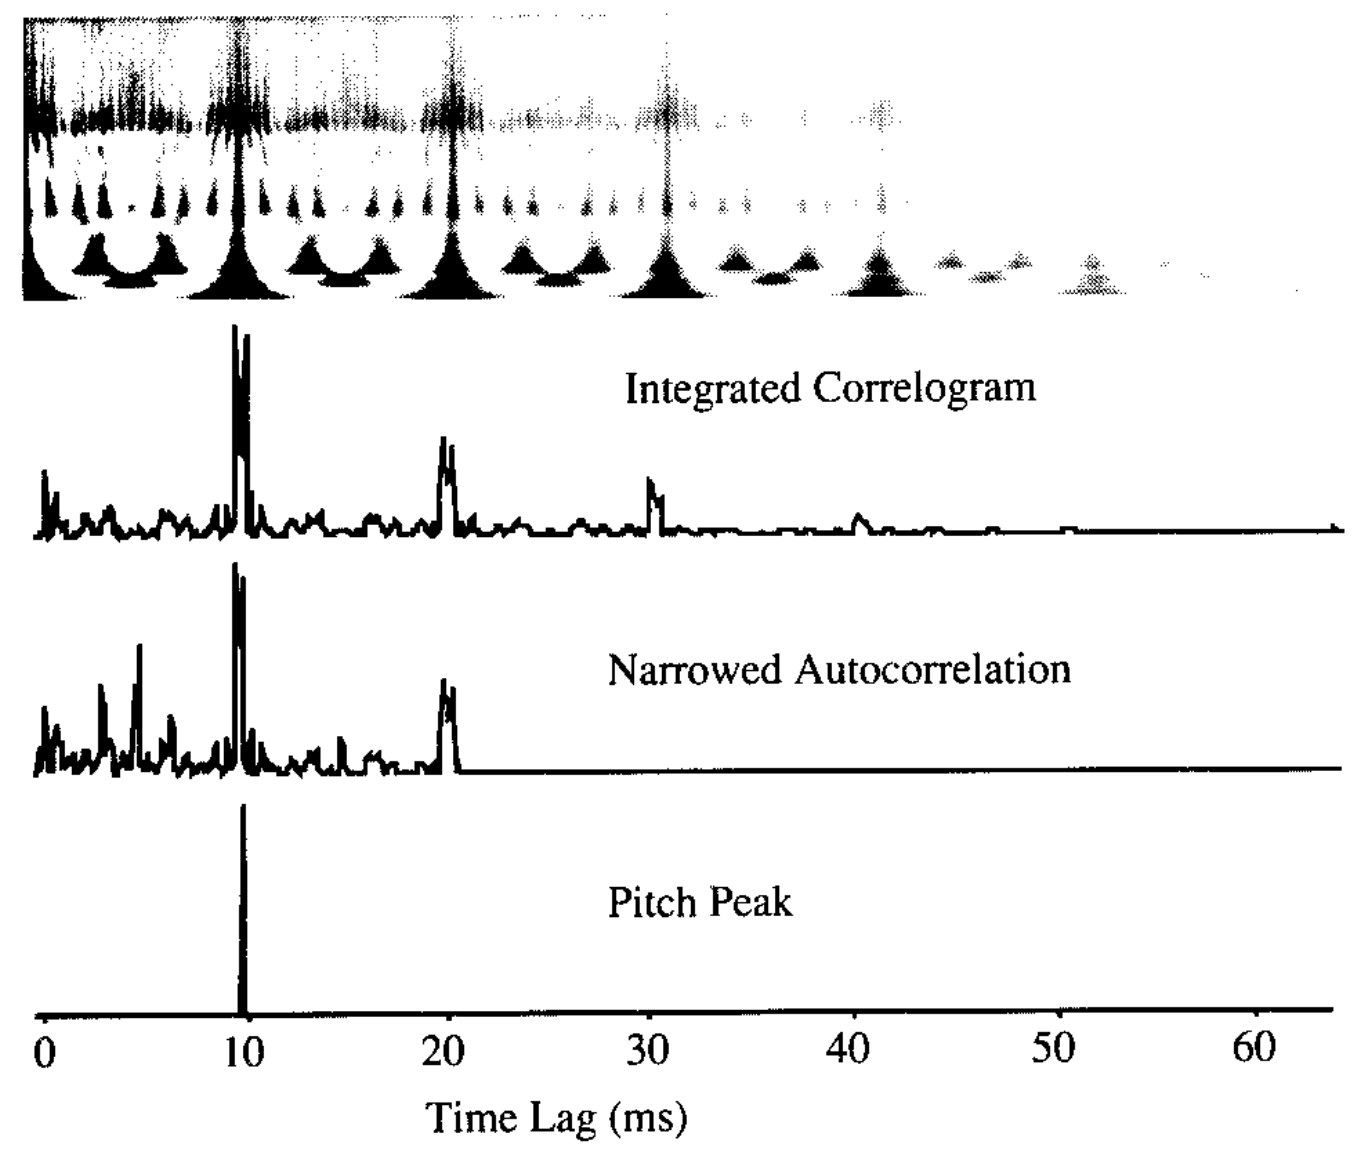
\includegraphics[width=0.7\textwidth]{slaney1990fig3.png}}
\end{frame}

\begin{frame}
  \frametitle{The SIFT pitch tracking algorithm}

  Markel (1972) proposed a pitch tracking algorithm called SIFT
  that was the basis of most pitch tracking algorithms since then:
  \begin{enumerate}
  \item Lowpass filter the signal to eliminate high-frequency noise
  \item Compute the autocorrelation, and find its first peak
  \item That's the pitch period!
  \end{enumerate}
\end{frame}

\begin{frame}
  \begin{columns}
    \begin{column}{0.5\textwidth}
      Autocorrelation can even find the pitch of a sine wave embedded
      in lots of noise, like the one at right
    \end{column}
    \begin{column}{0.5\textwidth}
      \centerline{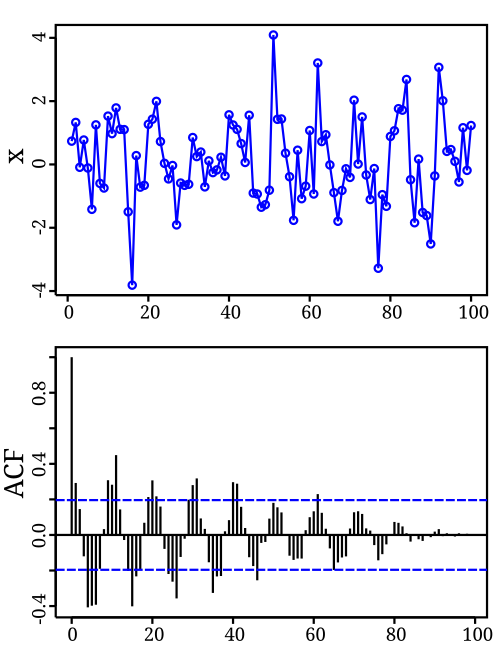
\includegraphics[width=\textwidth]{Acf_new.svg.png}}
      \centerline{\tiny{\url{https://commons.wikimedia.org/wiki/File:Acf_new.svg}}}
    \end{column}
  \end{columns}
\end{frame}

%%%%%%%%%%%%%%%%%%%%%%%%%%%%%%%%%%%%%%%%%%%%%%%%%%55
\section{Summary}

\begin{frame}
  \frametitle{Summary}

  \begin{itemize}
    \item Complex exponential, $x[n]=Ae^{j(\omega_0 n+\theta)}$:
      \begin{align*} r_x[n]=|A|^2 e^{-j\omega_0 n} r_w[n]
        &\Rightarrow |X(\omega)|^2=|A|^2|W(\omega-\omega_0)|^2
      \end{align*}
      \item 
        Complex tone, $x[n]=\sum_{k}X_kw[n]e^{j\frac{2\pi kn}{N_0}}$:
        \begin{align*}
          r_x[n]&\approx \sum_{k}|X_k|^2r_w[n]e^{j\frac{2\pi kn}{N_0}}\\
          &\Rightarrow |X(\omega)|^2 \approx 
          \sum_{k}|X_k|^2\left\vert W\left(\omega-\frac{2\pi kn}{N_0}\right)\right\vert^2
        \end{align*}
  \end{itemize}
\end{frame}


\end{document}
